\chapter{Base de datos e implementación}
\label{chap:implementación}


\section{Creación y modificaciones de la base de datos}

\subsection{Creación de la base de datos}

Para crear la base de datos se ha utilizado la herramienta de Supabase. Esta herramienta permite crear una base de datos y sus tablas correspondientes de forma sencilla. Además, tiene una fácil integración con Flutter, por lo que conectar la aplicación a la base de datos no fue complicado. Fue suficiente con añadir librerías y las claves de configuración.  

Una vez configurada la base de datos dentro del proyecto, se genera una instancia que se utilizará cada vez que sea necesario hacer operaciones en la base de datos: 

\begin{figure}[H]
	\centering
	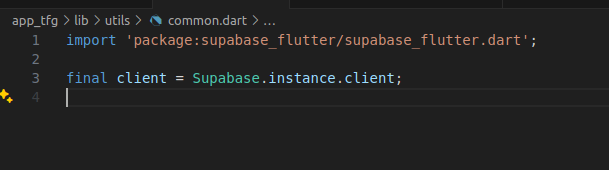
\includegraphics[width=0.7\textwidth]{imagenes/clientBD.png}
	\caption{Instancia de la base de datos.}
	\label{fig:instanciaBD}
\end{figure}

\newpage

\subsection{Tablas de la base de datos}

Las tablas que están dentro de la base de datos son: 


\begin{itemize}
	\item \textbf{clientes:} En esta tabla se almacena toda la información relativa a los clientes. Podemos encontrar campos como el nombre, el teléfono, un comentario para añadir más información y una cartera, que permitirá que el cliente pueda tener dinero negativo o positivo en la tienda. 
	\item \textbf{categorias:} En esta tabla se crean categorías para organizar los artículos dentro de la tienda. Sus atributos tieneTamanio, tieneDescripcion, tieneMaterial, tieneGenero, son booleanos que permiten personalizar los atributos que tendrá un artículo. Si no se seleccionan alguno de estos atributos, todos los artículos que se creen bajo esa categoría no tendrán ese atributo. El atributo nombre indica el nombre de la categoría. 
	\item \textbf{articulos:} En esta tabla se almacena la información de cada uno de los artículos de la tienda. Sus atributos fijos son el nombre, el precio y la subcategoría (que permite categorizar más fino dentro de una categoría y posteriormente filtrar por dichas subcategorías). El resto de atributos son opcionales y se elegirán en la creación de la categoría de dicho artículo. Un artículo representa un modelo, dentro de una prenda podrán haber varias tallas o varios colores, lo que se contempla en la siguiente tabla. 
	\item \textbf{tallas:}  En esta tabla se registran las tallas y los colores disponibles de cada uno de los artículos. Para cada talla se especifica un color, la cantidad actual y la cantidad mínima. La cantidad mínima sirve para detectar cuando un artículo necesita ser renovado. Cuando se tienen igual o menos artículos de los especificados en la cantidad mínima, se mete en una lista de renovación de stock para indicar que deben ser renovados. 
	\item \textbf{movimientos:} En esta tabla se registra toda la información relacionada con los movimientos de la tienda. Se registra el precio total del movimiento, el cliente asignado, el método de pago, la fecha, el tipo de movimiento y el movimiento anterior, este atributo sirve para relacionar unos tickets con otros. Cuando se hace una devolución, se le asigna el movimiento anterior del que procede para poder ver cuál es su procedencia. Además, a las ventas / préstamos también se le asignan las devoluciones para una mejor sincronización.  
	\item \textbf{articulosMov:} En esta tabla se registran todos los artículos que pertenecen a cada movimiento. Es la tabla resultante de una relación muchos a muchos. Además, también se almacena como información adicional, la cantidad comprada de esa talla y el precio parcial. 
\end{itemize}


\subsection{Modificaciones intermedias de la base de datos}

Debido al cambio que solicitó el cliente con las tallas, se tuvo que crear una nueva tabla, la tabla tallas. Esto permitió que un artículo pudiera tener distintas tallas o distintos colores. 


\subsection{Diagrama final del diseño de la base de datos}

En este diagrama podemos ver los atributos que posee cada una de las tablas y como se relacionan entre ellas. Las líneas discontinuas indican las claves externas y los atributos con la llave a la izquierda representan las claves primarias de cada tabla. 

\begin{figure}[H]
	\centering
	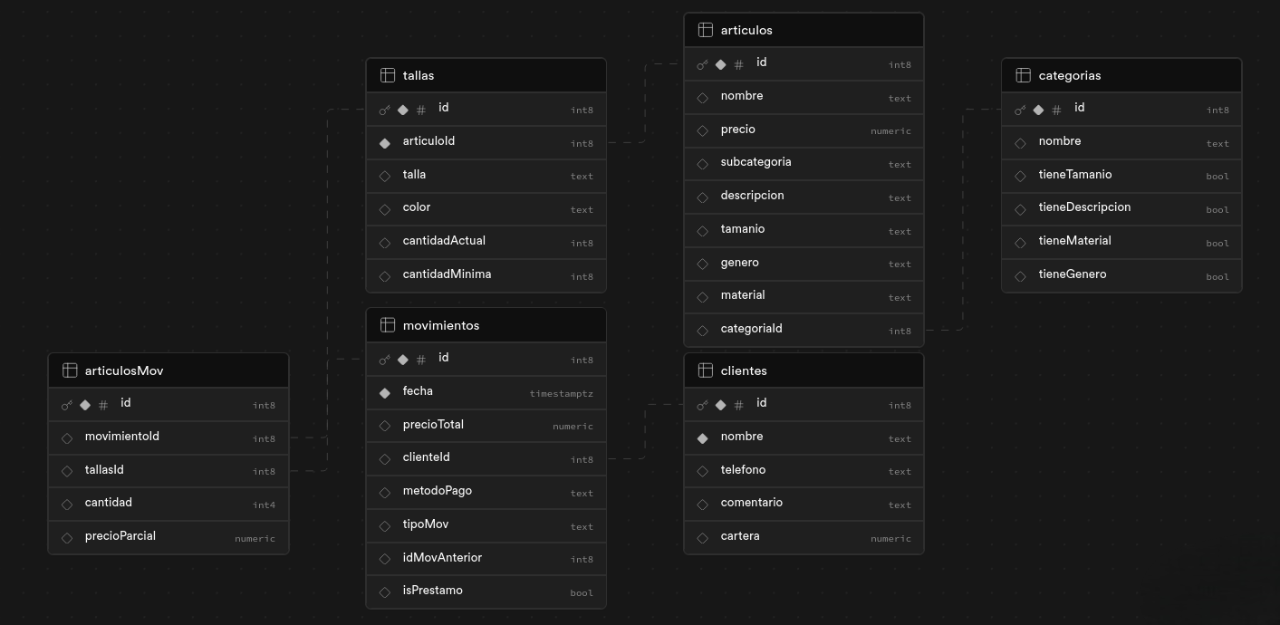
\includegraphics[width=0.7\textwidth]{imagenes/imagenesDiagramas/diagramaBD.png}
	\caption{Diagrama de la base de datos.}
	\label{fig:diagramaBD}
\end{figure}

\section{Diagrama de clases}

Tras finalizar la implementación de la aplicación, se ha construido un diagrama de clases para poder observar las clases que componen el proyecto y las relaciones entre estas. También se pueden ver los atributos y los métodos que tiene cada una de las clases. 

\newpage

\begin{figure}[H]
	\centering
	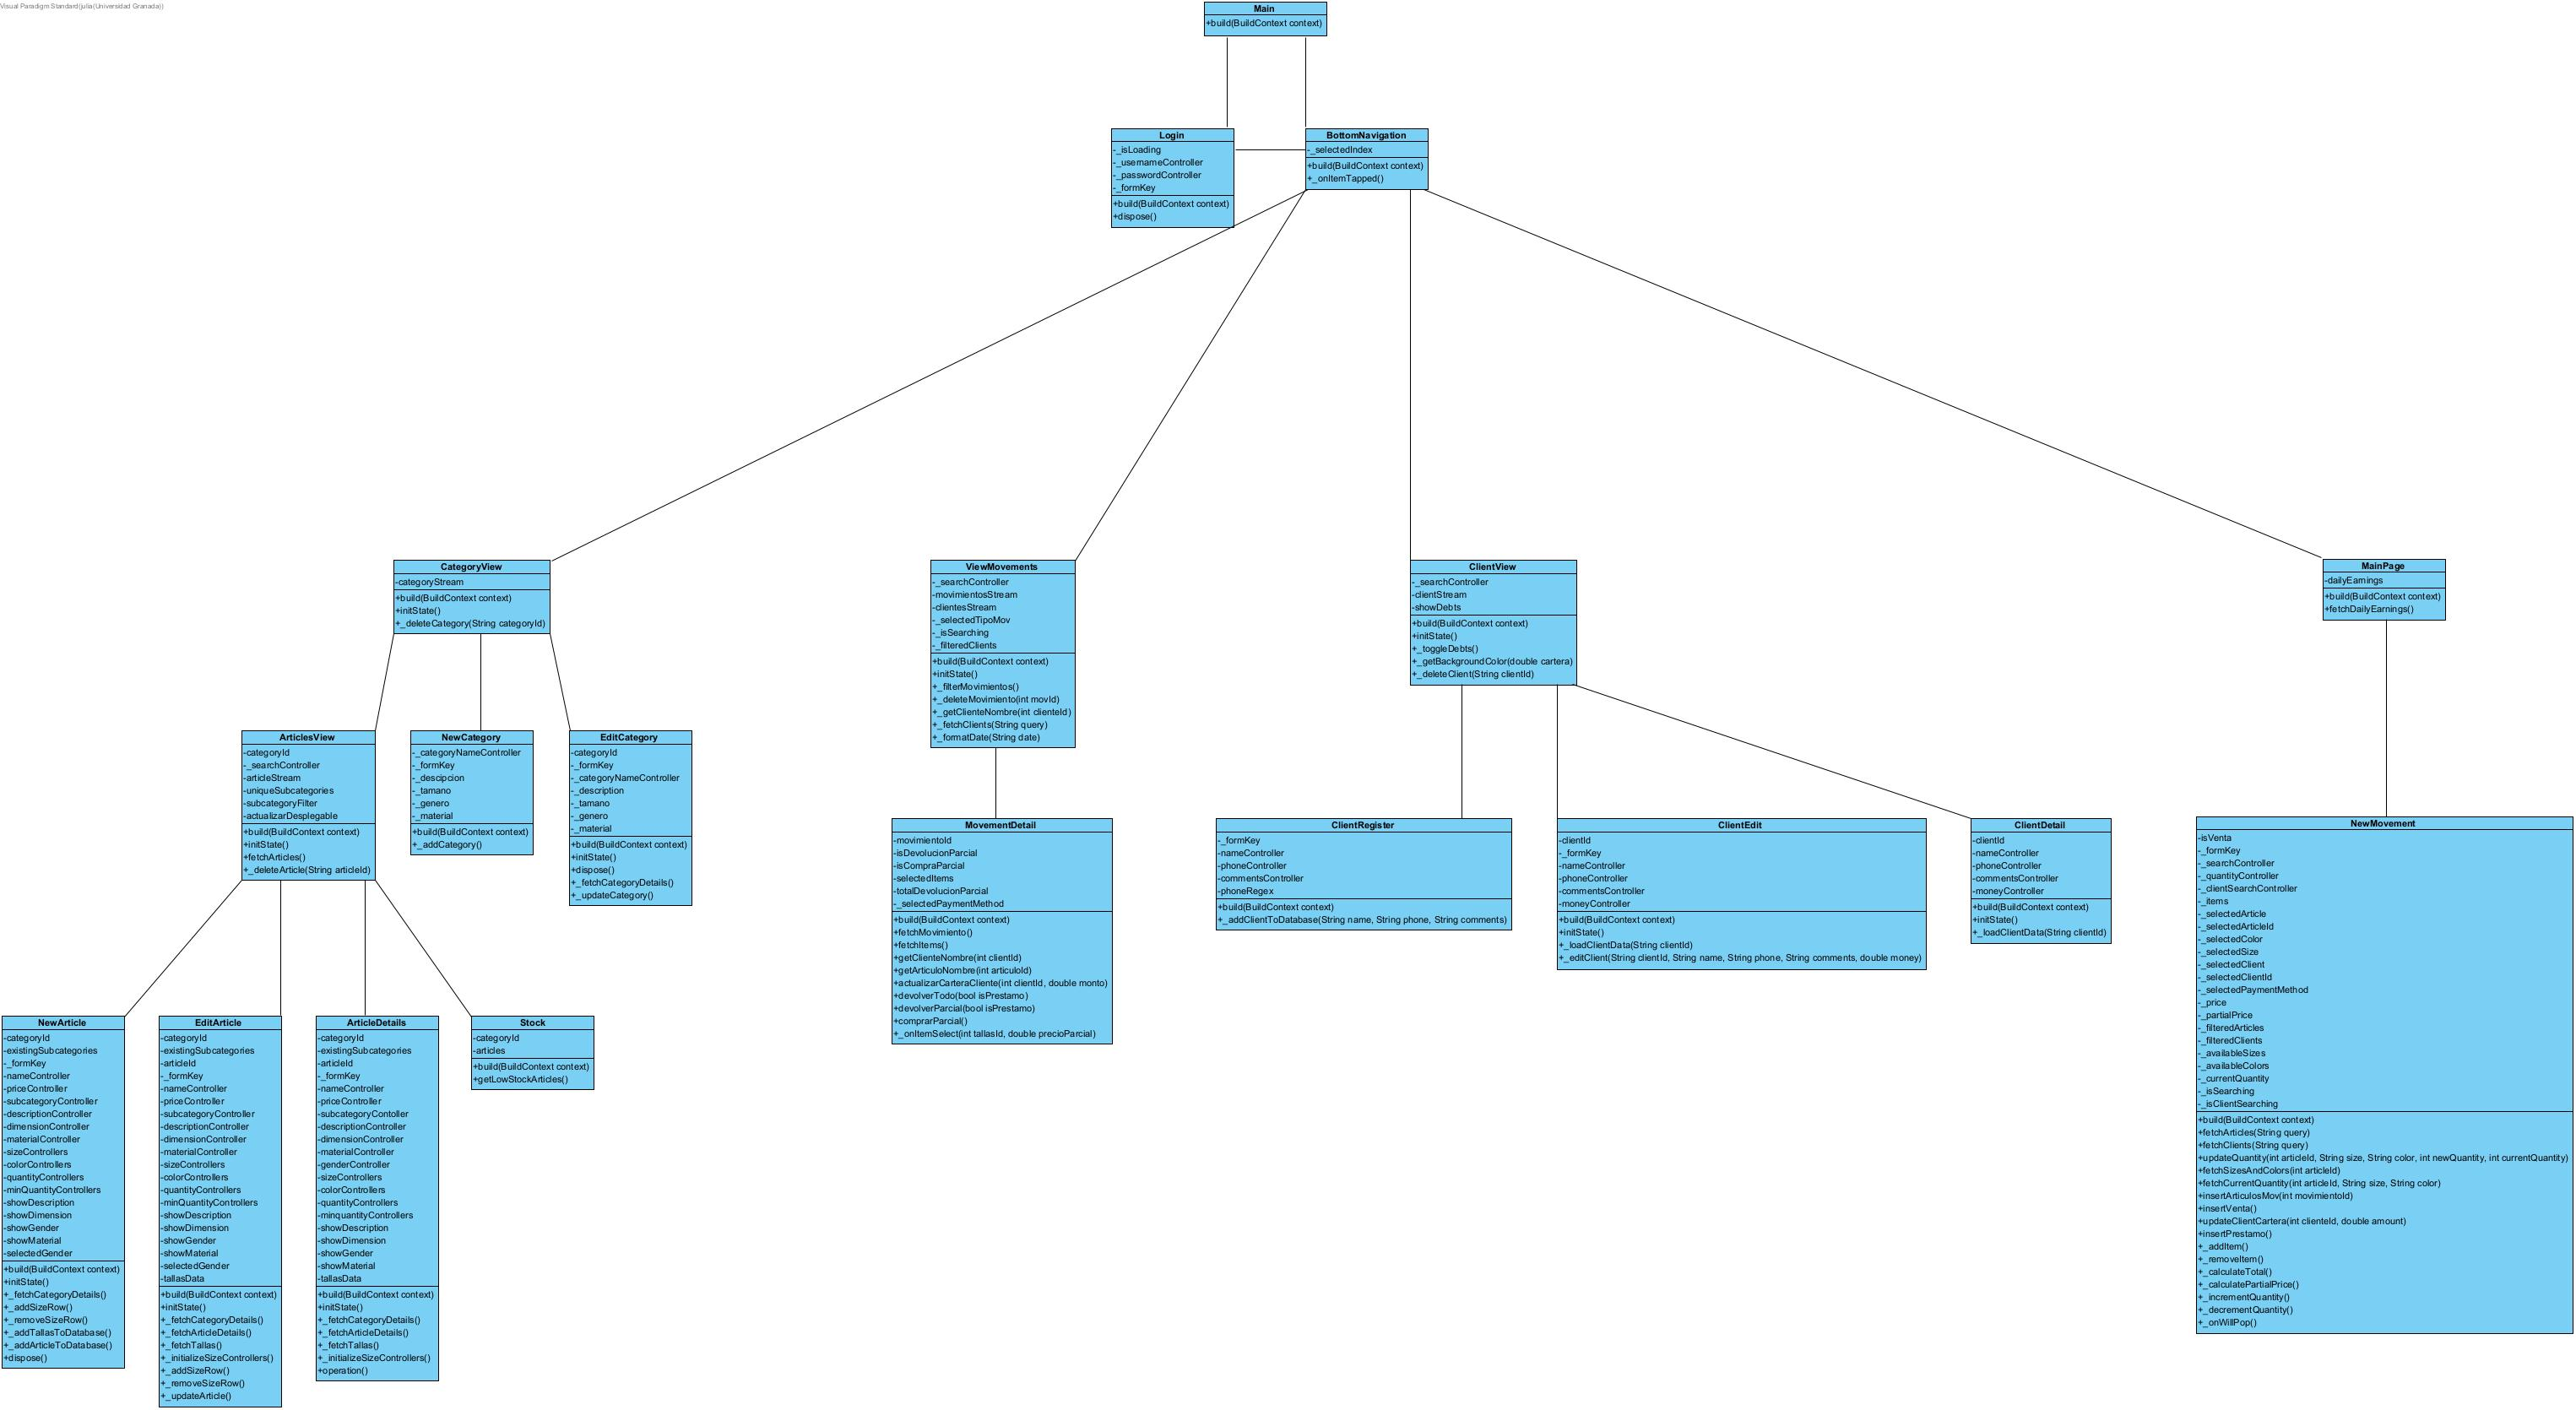
\includegraphics[width=1.1\textwidth, angle=180]{imagenes/imagenesDiagramas/diagramaClases.jpg}
	\caption{Diagrama de clases.}
	\label{fig:diagramaClases}
\end{figure}
